%%%%%%%%%%%%%%%%%%%%%%%%%%%%%%%%%%%%%%%%
%    INSTITUTE OF PHYSICS PUBLISHING 
%   `Preparing an article for publication in an Institute of Physics
%    Publishing journal using LaTeX'
%    LaTeX source code `ioplau2e.tex' used to generate `author guidelines', the documentation explaining and demonstrating use of the Institute of Physics Publishing LaTeX preprint files       %
%    `iopart.cls, iopart12.clo and iopart10.clo'.
%    `ioplau2e.tex' itself uses LaTeX with `iopart.cls'
%%%%%%%%%%%%%%%%%%%%%%%%%%%%%%%%%%

\documentclass[10pt]{iopart}
\newcommand{\gguide}{{\it Preparing graphics for IOP Publishing journals}}
%Uncomment next line if AMS fonts required
%\usepackage{amsmath}
\usepackage{iopams}
\newcommand{\m}{\textup{\texttt{-}}}
\usepackage{graphicx}
\graphicspath{{figures/}}
\usepackage{color}
\newcommand{\revision}[1]{\color{red} {#1}}
\usepackage{url}
%\usepackage{hyperref}
\begin{document}

\title[Power spectrum scaling as a measure of critical slowing down]{Power spectrum scaling as a measure of critical slowing down and precursor to tipping points in dynamical systems}

\author{Joshua Prettyman; Tobia Kuna; Valerie Livina}

\address{}
\ead{j.prettyman@icloud.com}
\vspace{10pt}
\begin{indented}
	\item[] October 2021
\end{indented}

\begin{abstract}
Many dynamical systems experience sudden shifts in behaviour known as tipping points or critical transitions, often preceded by the ``critical slowing down'' (CSD) phenomenon whereby the recovery times of a system increase as the tipping point is approached. Many attempts have been made to find a tipping point indicator: a proxy for CSD, such that a change in the indicator acts as an early warning signal. Several generic tipping point indicators have been suggested, these include the power spectrum (PS) scaling exponent whose use as an indicator has previously been justified by its relationship to the well-established detrended fluctuation analysis (DFA) exponent. {\revision In this paper we justify the use of the PS indicator analytically, by considering a mathematical formulation of the CSD phenomenon}. We assess the usefulness of estimating the PS scaling exponent in a tipping point context when the power spectrum does not exhibit power-law scaling, or changes over time. In addition we show that this method is robust against trends and oscillations in the time series, making it a good candidate for studying resilience of systems with periodic oscillations which are observed in ecology and geophysics. 
\end{abstract}


% Uncomment for keywords
%\vspace{2pc}
%\noindent{\it Keywords}: XXXXXX, YYYYYYYY, ZZZZZZZZZ
% Uncomment for Submitted to journal title message
\submitto{\ERL}
% Uncomment if a separate title page is required
%\maketitle
% For two-column output uncomment the next line and choose [10pt] rather than [12pt] in the \documentclass declaration
\ioptwocol


\section{Introduction}
\label{sec:Intro}

The phenomenon of critical slowing down (CSD) is observed in a broad range of dynamical systems exhibiting tipping behaviour~\cite{scheffer2001,lenton2008,scheffer2009,scheffer2009critical, dakos2011slowing}. The `slowing down' to which the phrase refers is the increasing times taken by the system to return to the equilibrium state given a random perturbation: at some \emph{critical} point (a tipping point) the system changes state and the return time becomes effectively infinite. The autocorrelation scaling exponent of time series data is a useful measurement of CSD~ \cite{scheffer2009critical} and is a candidate for use as a tipping point indicator. The closely related detrended fluctuation analysis (DFA)~\cite{kantelhardt2001,livina2007} and power spectrum (PS)~\cite{prettyman2018,prettyman2019} scaling exponents have also been used as indicators following the `degenerate fingerprinting' technique of Ref.~\cite{held2004}. It is, however, tacitly assumed that the estimation of the PS scaling exponent will yield a useful tipping point indicator (although this is not obvious when the power spectrum does not actually exhibit true power-law scaling). In this paper we demonstrate that the PS scaling exponent is relevant to the AR(1) model of CSD, which has a non-scaling power spectrum, and demonstrate that the method is resilient to oscillations in the underlying dynamical system. 

In Sec.~\ref{sec:modellingCSD} we examine the PS scaling exponent of the lag-1 autoregressive (AR(1)) process which is used as a model of critical slowing down. In Sec.~\ref{sec:frequencyRange} we then look more closely at the PS indicator method to determine the best frequency range by which to estimate the exponent for a power spectrum not exhibiting power-law scaling.


In Sec.~\ref{sec:noTrueScaling} we apply this method of estimating the PS exponent to data for which the power spectrum does not exhibit power-law scaling and, in Sec.~\ref{sec:sensitivity}, we model a system undergoing CSD by considering AR(1) processes with increasing autoregressive parameter and analyse the sensitivity of the estimated PS exponent to the size of the data set and the addition of trends and periodicities to the AR(1) process. This is particularly relevant to measuring resilience in ecological or geophysical systems with complex periodicities which may be difficult to remove.

Finally in Sec.~\ref{sec:gisp-ice-core} we consider an application of this method to paleo-temperature proxy data previously found to exhibit tipping behaviour \cite{lenton2012climate}.

\section{A model of critical slowing down}
\label{sec:modellingCSD}

The use of the autocorrelation scaling exponent as a tipping point indicator is justified by modelling a one-dimensional dynamical system using a lag-1 autoregressive (AR(1)) process~\cite{held2004, scheffer2009}:
\begin{equation}
	\label{eqn:1D:AR1_decay_model}
	{\revision z(t_{n+1}) = e^{-\kappa\Delta t}z(t_{n}) + \sigma\eta_n \,, }
\end{equation}
{\revision where $\sigma$ is a constant, $\Delta t = t_{n+1} - t_n$, $\eta_n$ is a white noise term and $\kappa$ is the decay rate.} The model considers the equilibrium state $z=0$ as the critical mode of a dynamical system undergoing a bifurcation. The system returns to equilibrium exponentially with rate $\kappa$. During a bifurcation a system will undergo critical slowing down, that is, a decreasing rate $\kappa$. The autocorrelation coefficient $\alpha \equiv e^{-\kappa\Delta t}$ increases to $1$ as $\kappa$ decreases to zero. The autoregressive model parameter $\exp(-\kappa\Delta t)$, and thus the simple lag-1 autocorrelation function (ACF1), will increase as $\kappa$ decreases. The ACF1 is therefore a good tipping point indicator and is widely used~\cite{held2004,lenton2012}. As noted by Ref.~\cite{scheffer2009}, it is often the case that as the autocorrelation increases so does the variance, this is true of the AR(1) process described by Eqn.~\ref{eqn:1D:AR1_decay_model} where the expectation is zero and the variance is given by
\begin{equation}
	\textrm{Var}(z(t)) = \frac{\sigma^2}{1-\mu^2}\,,
\end{equation} 
where $\mu=\exp(-\kappa\Delta t)$ is the autocorrelation coefficient. Thus detecting an increase in variance will provide an additional early warning signal.

The PS exponent $\beta$ of a time series $x(t)$, as used in Ref.~\cite{prettyman2019} as a tipping point indicator, is defined as the negative power-law scaling exponent of the power spectral density (PSD), which is the modulus squared of the Fourier transform. This is, if the PSD of the process $x(t)$ satisfies the power-law scaling relationship
\begin{equation}
	\label{eqn:1D:power_spectrum_def}
	S_x(f) := \left|\int_{\m \infty}^{\infty} x(t) e^{\m 2\pi i f t} dt\right|^2\sim f^{-\beta}\,,
\end{equation}
then we define $\beta$ as the PS exponent. If the PSD is obtained numerically as the fast Fourier transform periodogram~\cite{prettyman2018,prettyman2019}, then $\beta$ must be estimated by plotting the periodogram on logarithmic axes and measuring the negative gradient, expressed in terms of the PSD as 
\begin{equation}
	\beta_f = -\frac{d}{d(\log f)}\log\left[S_x(f)\right]\,\
	\label{eqn:PSD_derivative}
\end{equation}
(where `$\log$' refers to the base-$10$ logarithm) which is a constant in terms of $f$ only if the PSD exhibits true power-law scaling (a straight line in the log-log plot). In practice a single value for $\beta$ is obtained by using a linear fit to the periodogram either over the entire frequency range $f\in(0,0.5]$ or in some subset $\log f\in[a_1, a_2]$ where $a_1<a_2\leq\log(0.5)$. That is, we find the linear function $p:\log f\mapsto\beta\log(f)+c$ minimizing the squared error
\begin{equation}
	\sum_{a_1 \leq \log f\leq a_2} |p(\log f) - \beta_f|^2.
	\label{eqn:beta_integral}
\end{equation}
In cases where the power spectrum does not exhibit power-law scaling the choice of the frequency range is a significant consideration potentially affecting the usefulness of the estimated value $\beta$ as a tipping point indicator. In Sec.~\ref{sec:frequencyRange} we analyse the PS exponent more closely in an EWS context in order to ascertain optimal values of $a_1$ and $a_2$. 


\section[PS exponent frequency range]{Determining the frequency range for the PS exponent estimation}
\label{sec:frequencyRange}

When estimating the value of the PS scaling exponent from a discrete periodogram it is necessary to use a chosen range of frequencies for the calculation (the $a_1$ and $a_2$ in Eqn.~\ref{eqn:beta_integral}) since at very high or low frequencies the discrete periodogram will not be reliable. In particular, very low frequencies do not exist in the discrete periodogram and the range of frequencies available is determined by the length of the time series (i.e. the number of data) used. In previous work~\cite{prettyman2019, prettyman2021} we have calculated the exponent over the range $10^{\m2} \leq f \leq 10^{\m1}$ since this relates to the time range $10 \leq s \leq 100$ used in the estimation of the DFA scaling exponent as presented by Ref.~\cite{livina2007}. 

In cases where true power-law scaling exists, and data exist with sufficiently high time resolution, the estimation can be done over any sensible range, or over the entire periodogram. Where there is no true power-law scaling, the choice of the range of frequencies may significantly affect the result. For our purposes, where the value of the scaling exponent is used as an early warning signal of a tipping point, it is not the exponent value itself in which we are interested but the \emph{change} in the exponent as the system approaches a tipping point. In this section we find a rule-of-thumb frequency range for the exponent estimation by examining a model of the CSD phenomenon (an AR(1) process with increasing AR parameter) and determining the range of frequencies in which the periodogram shows most consistent and visible change. 


In this paper we follow Ref.~\cite{scheffer2009} in using the AR(1) process $z_{n+1} = \mu z_n +\sigma\eta_n$, with increasing parameter $\mu$, as a model of a process experiencing CSD. The autoregressive parameter $\mu$ is therefore considered to be a function of time $t$ and is assumed to be monotonically increasing. In our attempt to analyse the power spectral properties of CSD processes we therefore consider the PSD of the AR(1) process, which is given in Ref.~\cite{vonstorch} as
\begin{equation}
	\label{eqn:1D:PSindicator:AR1powerspectrum}
	S_z(f) = \frac{\sigma^2}{1+ \mu^2 - 2\mu\cos(2\pi f)}\,.
\end{equation}
The specific power spectrum exponent $\beta_f$ is then found, as in Eqn.~\ref{eqn:PSD_derivative}, by differentiating $\log[S_z(f)]$ with respect to $\log f$:
\begin{eqnarray}
	\beta_f &= -\frac{d}{d(\log f)}\log[S_z(f)]\\
	&= \frac{4\pi \mu f \sin(2\pi f)}{1+\mu^2-2\mu\cos(2\pi f)}\,.
	\label{eqn:PSE_calculation}
\end{eqnarray}
This gradient may then be evaluated at a particular value of $f$ (or, rather, in the case of the periodogram, estimated by a linear fit in a particular range of $f$ values). What we refer to as the \emph{Power Spectrum Indicator} is the value of this PS exponent as a function of time, $B_f(t)$, given by the expression in Eqn.~\ref{eqn:PSE_calculation}, where the $t$ dependence comes from the fact that $\mu = \mu(t)$ is a function of time. That is,
\begin{equation}
	\label{eqn:1D:PSindicator_AR1}
	B_f(t)= \frac{4\pi \mu(t) f \sin(2\pi f)}{1+\mu(t)^2-2\mu(t)\cos(2\pi f)}\,.
\end{equation}
In the following calculations we instead consider the PS indicator directly as a function of $\mu$, which can be done without loss of generality assuming $\mu(t)$ is increasing. Taking the $\mu$ derivative we find
\begin{equation}
	\frac{d}{d\mu}B_f(\mu) = \frac{4\pi f \sin(2\pi f)(1-\mu^2)}{\left(1+\mu^2-2\mu\cos(2\pi f)\right)^2}.
\end{equation}
Equating this to zero we find the maximum value of the PS indicator occurs when $\mu=1$ (when the AR(1) process is a random walk) at which point the PS indicator $B_f$ has a maximal value of 2 which occurs as $f$ approaches zero, that is,
\begin{equation}
	\label{eqn:1D:maximumPSindicator_AR1}
	\max[B_f] = B_f(1) = \frac{2\pi f \sin(2\pi f)}{1-\cos(2\pi f)} ~\rightarrow~ 2\,.
\end{equation}
For larger values of $f$ the maximum indicator value is not close to the maximal value of 2. For $f = 0.1$ we have $B_{0.1}(1) = 1.93$, whereas for $f = 0.38$ already the value is significantly less:  $B_{0.38}(1) = 1$ (note that $B_{1/2}(1)=0$). In cases where the PS indicator is being estimated using a noisy periodogram it is essential that the increase in the indicator value as critical slowing down occurs (that is, as $\mu$ increases from 0 to 1) is easily observable. For this reason, when we estimate the PS scaling exponent, a frequency $\log(f)\leq \m1$ should be used in order to be able to observe the largest increase in the PS indicator.

\begin{figure} % FIGURE 2.10 from Thesis
	\centering
	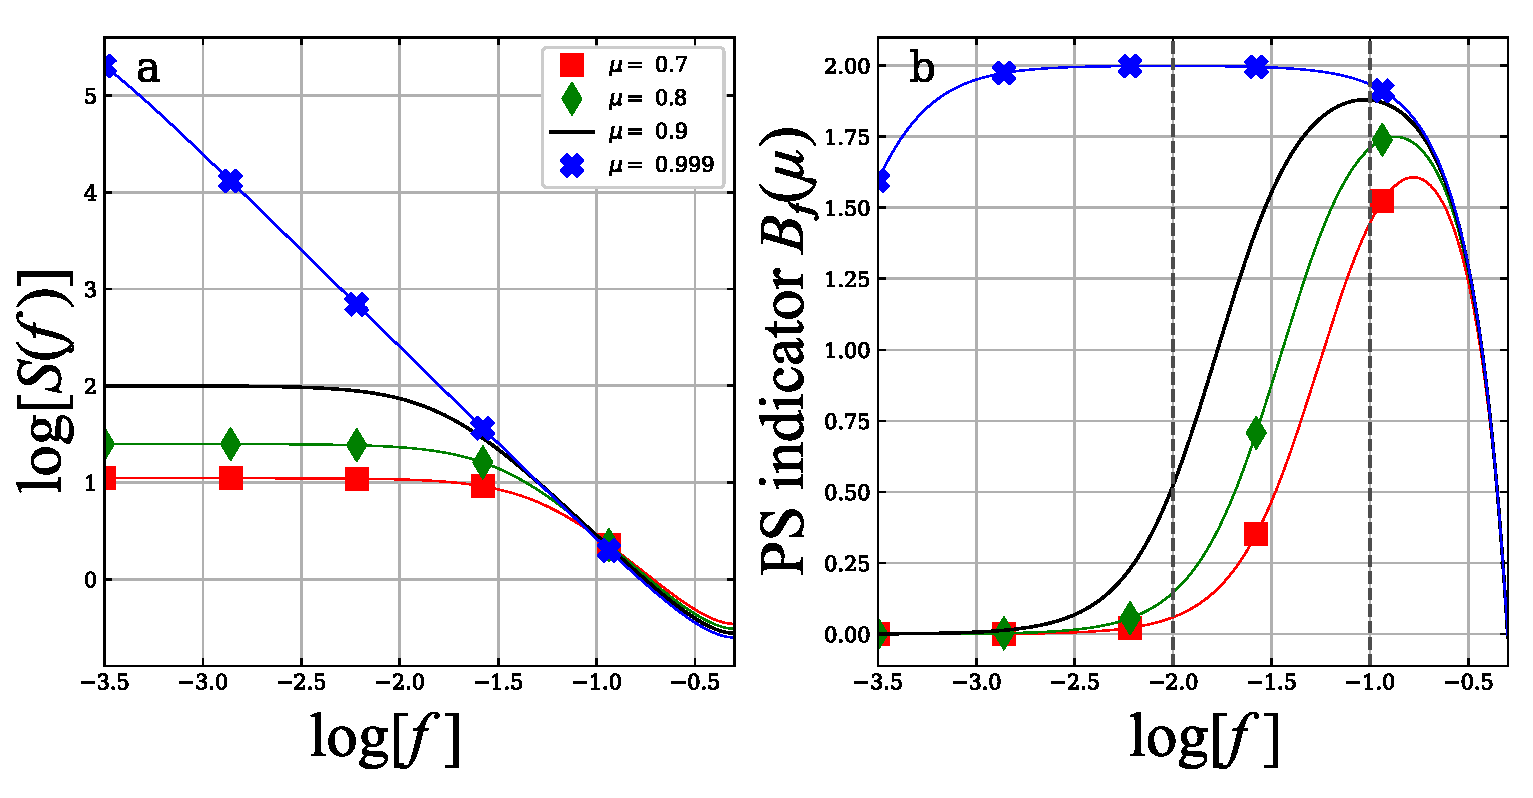
\includegraphics[width=0.95\linewidth]{c2fig10}
	\caption{\label{fig:AR1PowerSpectrum}
		{Scaling properties of the AR(1) process with varying parameter $\mu$. Panel~{\bf a}: The power spectrum of the AR(1) process (see Eqn.~\ref{eqn:1D:PSindicator:AR1powerspectrum}) is plotted on a log-log scale for various values of the parameter $\mu$. Note the `white-noise' (flat) part of the power spectrum for small $f$ and the 'red-noise' (negative gradient) part for large $f$. Panel~{\bf b}: The PS indicator (see Eqn.~\ref{eqn:1D:PSindicator_AR1}) is plotted as a function of $f$ for the same $\mu$ values.}
	}
\end{figure}

In Fig.~\ref{fig:AR1PowerSpectrum} the PSD of the AR(1) process, as given by Eqn.~\ref{eqn:1D:PSindicator:AR1powerspectrum}, is plotted for parameter $\mu = 0.7, 0.8, 0.9, 0.999$ (Panel {\bf a}). We note that for $\mu=0.999$ the AR(1) process is very similar to a random walk ($\mu=1$) and thus the power spectrum clearly exhibits the associated negative gradient in the log-log plot. For lower values of $\mu$, where the process is somewhere between a white noise process ($\mu =0$) and a random walk, we note that a ``cross-over'' occurs in the range $\m2<\log(f)<\m1$ (that is, there is a flat `white noise' power spectrum for low frequencies and a negative-gradient 'random walk' spectrum for higher frequencies) suggesting that this is the range in which the PS exponent (the gradient of the PSD plots) will exhibit the most noticeable change. Indeed, the PS exponent in the range $\m3.5<\log(f)<\m2.5$ is close to zero for all $\mu<0.9$, only exhibiting a change for $\mu \in [0.9, 1.0]$, and so cannot provide a useful indicator of CSD which is usually modelled as an increase of $\mu$ from $0$ to $1$. 

We note that there may be specific cases where a greater degree of sensitivity is required, for example where the CSD can be modelled as an increase in $\mu$ between $0.9$ and $1.0$. This may arise if the time series under investigation has a high ($\mu \approx 0.9$) ``background'' autocorrelation to start with. In this case, if the resolution of the time series is high enough that the periodogram is sufficiently reliable for low frequencies, a lower frequency range, such as $\m3.5<\log(f)<\m2.5$, might yield a more effective tipping point indicator. Alternatively, a Gaussian filter may be applied.

In Fig.~\ref{fig:AR1PowerSpectrum}{\bf b} we plot the PS indicator $B_f(\mu)$ as a function of $f$ and note again that the most significant increase in $B_f(\mu)$ as $\mu$ increases from $0$ to $1$ (comparing successive lines in the plot) is found in the frequency range $\m2<\log(f)<\m1$, i.e. $10\leq s\leq 100$.




\section{Estimating the PS exponent for power spectra without power-law scaling}
\label{sec:noTrueScaling}

The definitions of all scaling exponents, and thus it seems that the resulting early warning indicators, assume the existence of power-law scaling. For example, in the case of the PS exponent we assume the power spectrum $S(f)$, which is approximated by the periodogram, is of the form $S(f)\sim f^{-\beta}$ for some exponent $\beta$, and it is this value that we seek to measure. However, it is unlikely that we will find true power-law scaling like this in dynamical systems or data from real-life processes unless we are dealing with pure white noise or a pure random walk. Indeed we note that the common stochastic model, the AR(1) process, with which we model critical slowing down~\cite{scheffer2009critical}, does not even have true asymptotic power-law scaling in the power spectrum, as shown in Fig.~\ref{fig:AR1PowerSpectrum}.

In this section we show that it is still valuable to measure the PS exponent in cases in which there is clearly no true power-law scaling. In particular, we focus on two cases where the power spectrum has ``crossover'': a process for which the power spectrum follows one power-law scaling relationship at low frequencies and another at higher frequencies.
\begin{enumerate}
	\item The combination of a white noise series and a red noise series, in which the white noise signal dominates at the higher-frequency end of the power spectrum whilst the red noise dominates the low-frequency end.
	\item The aforementioned AR(1) process which has power spectrum described by Eqn.~\ref{eqn:1D:PSindicator:AR1powerspectrum} with parameter $\mu\in[0,1]$.
\end{enumerate}
In both of these cases we attempt to estimate a specific power spectrum scaling exponent $\beta_f$ by applying a linear fit to the non-linear log-log periodogram in some range $[f_0, f_1]\ni f$. We then show that this pseudo scaling exponent provides a proxy for increased `reddening' of the underlying process.

\subsection{Sum of red and white noise signals}

\begin{figure} % FIGURE 2.8 from Thesis
	\centering
	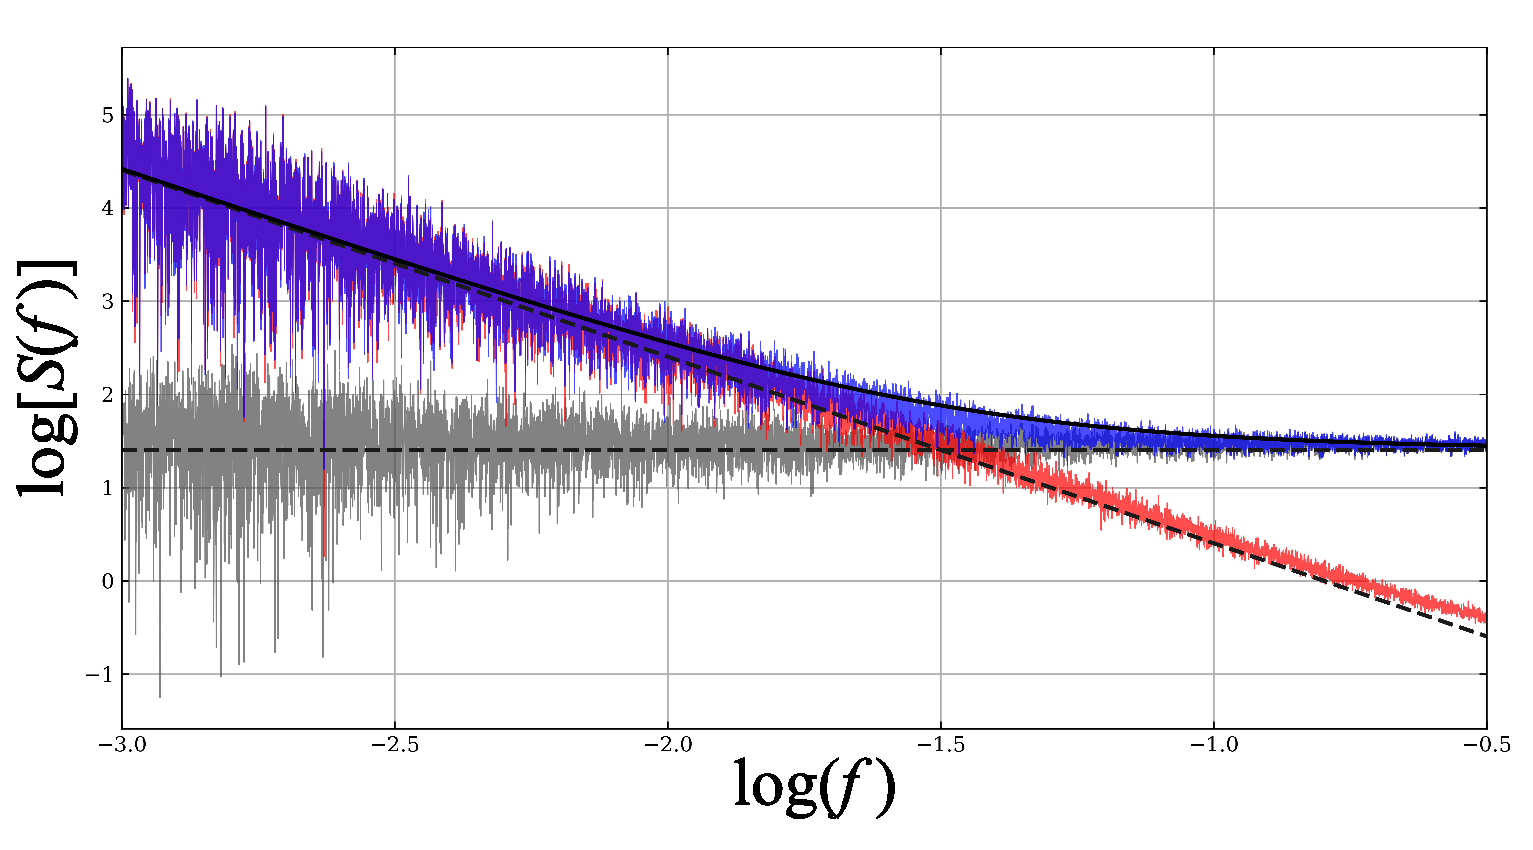
\includegraphics[width=0.95\linewidth]{c2fig08}
	\caption{\label{fig:1D:crossover1}
		{Scaling crossover in the power spectrum of the sum of red and white noise series. Showing the power spectrum of the series $z(t)$ (solid black line, see Eqn.~\ref{eqn:1D:crossoverfunction}) imposed over the periodogram (blue). Also showing the power spectrum of white and red noise (dashed black lines) and their periodograms (grey and red respectively). The crossover occurs at $f=10^{\m3/2}$.}
	}
\end{figure}

To create a time series with a clear crossover in the power spectrum we take the sum of a Gaussian white noise series $\eta_t$ and red noise (random walk) series $W_t$ defined by the relation $W_t = W_{t-1} + \zeta_t$, where $\zeta_t$ are a Gaussian white noise series independent of $\eta_t$. Thus the terms of the series are given by
\begin{equation}
	\label{eqn:1D:crossoverfunction}
	z(t) = \left(\sum_{\tau=0}^t \zeta_\tau\right) + \mu\eta_t\,,
\end{equation}
where $\mu$ is a parameter modifying the variance of the white noise terms $\eta_t$. Due to the linearity of the Fourier transform {\revision we are able to calculate the power spectral density $S_z(f)$ of the series $z(t)$ by combining the Fourier transform $\hat{\eta}(f)=1$ of the white noise process $\eta(t)$ and the Fourier transform $\hat{W}(f) = (2\pi f)^{\m1}$ of the red noise (Brownian) process $W(t)$. The derivation follows}:
\begin{equation}
	\label{eqn:1D:powerspectrum_white}
	S_{\mu\eta}(f) = \left| \mu\hat{\eta}(f) \right|^2 = \mu^2\,,
\end{equation}
and
\begin{equation}
	\label{eqn:1D:powerspectrum_red}
	S_{W}(f) = \left| \hat{W}(f) \right|^2 = \left|\frac{1}{2\pi f}\right|^2 = \frac{1}{4\pi^2}f^{\m2}.
\end{equation}
Combining the two series we have
\begin{eqnarray}
		S_z(f) &= \left| \hat{z}(f) \right|^2\nonumber\\
		&= \left| \hat{W}(f) + \mu\hat{\eta}(f) \right|^2\nonumber\\
		\label{eqn:1D:powerspectrum_cross}
		&= \frac{1}{4\pi^2}f^{\m2} + \frac{\mu}{2\pi}f^{\m1} + \mu^2\,.
\end{eqnarray}

In Fig.~\ref{fig:1D:crossover1} the power spectra of white noise $\mu\eta_t$ and red noise $W_t$, given by Eqns.~\ref{eqn:1D:powerspectrum_white} and~\ref{eqn:1D:powerspectrum_red} respectively, are shown (dashed lines) imposed over the periodograms of computed instances of these series (shown in grey and red respectively). In this case the value $\mu = 10^{3/2}/2\pi$ has been chosen so that the intersection of the two curves is given by $f = 10^{\m3/2}$, which is the midpoint of the values $f=0.01$ and $f=0.1$ on the logarithmic scale. 

In Fig.~\ref{fig:1D:crossover1} we also see the power spectrum of the function $z(t)$, given by Eqn.~\ref{eqn:1D:powerspectrum_cross} (solid line), and the periodogram of an instance of the time series (shown in blue). This time series is simply the sum of the white noise and red noise series. We note that the periodogram of $z$ entirely overlaps the periodogram of the red noise series $W$ for small values of $f$, and overlaps the periodogram of the white noise series $\eta$ for large values of $f$. 

\begin{figure}
	\centering
	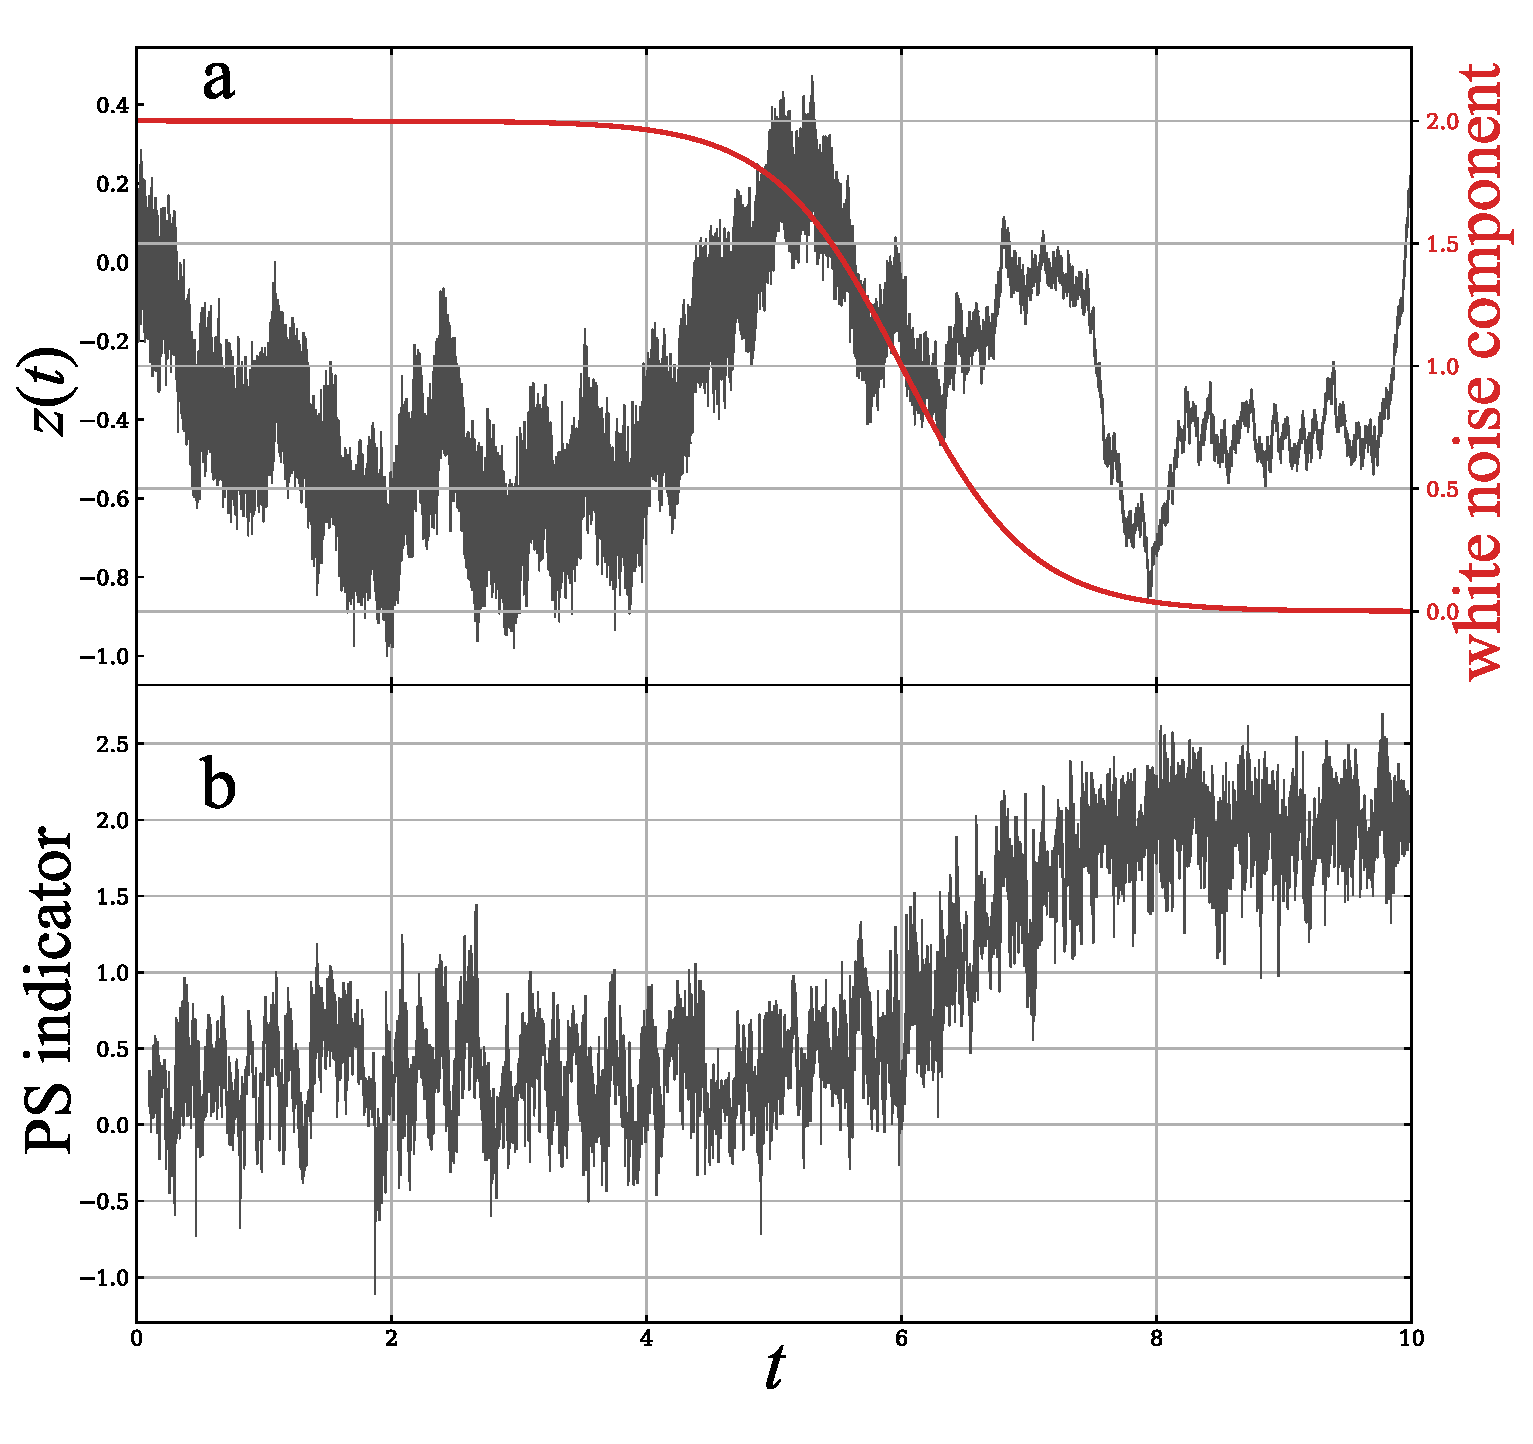
\includegraphics[width=\linewidth]{c2fig09}
	\caption{\label{fig:1D:crossover2}
		{Power spectrum indicator of the sum of white noise and red noise series with decreasing white noise component. Panel~{\bf a}: The time series $z(t)$ (left $y$-axis) and the standard deviation of the white noise component (right $y$-axis). Panel~{\bf b}: The PS indicator in a sliding window of size $1\%$ of the length of the time series.}
	}
\end{figure}

In Fig.~\ref{fig:1D:crossover2}{\bf a} we consider a time series $z(t)$ given by Eqn.~\ref{eqn:1D:crossoverfunction} but with a changing parameter $\mu$ given by:
 \begin{equation}
 	\mu(t) = 1 - \tanh(t - 6),
 \end{equation}
so that the value of standard deviation of the white noise component decreases from $2$ to $0$ as $t$ goes from $0$ to $10$, whilst the component random walk process is produced using a constant-variance white noise signal. In Fig.~\ref{fig:1D:crossover2}{\bf b} we plot the power spectrum indicator of the signal $z(t)$ and note that, whilst noisy (we are using a model ensemble of size 1), the PS indicator well reflects the change in the white noise component, rising synchronously as $\mu(t)$ decreases. The PS indicator in this case is calculated by estimating the PS exponent in the frequency range $\m2<\log(f)<\m1$, as determined in Sec.~\ref{sec:frequencyRange}. 

We have thus demonstrated the applicability of the PS indicator to a process whose power spectrum does not exhibit power-law scaling. By estimating the PS scaling exponent in the optimal frequency range we have detected the `reddening' of the noise signal. It is indeed this `reddening', or a shift from a process approximated by white noise towards a random walk, that characterises CSD, but it is the AR(1) process in particular which provides a model of this phenomenon~\cite{held2004, ashwin2012}.

\subsection{Power spectrum of the AR(1) process}


\begin{figure} % FIGURE 2.7 from Thesis
	\centering
	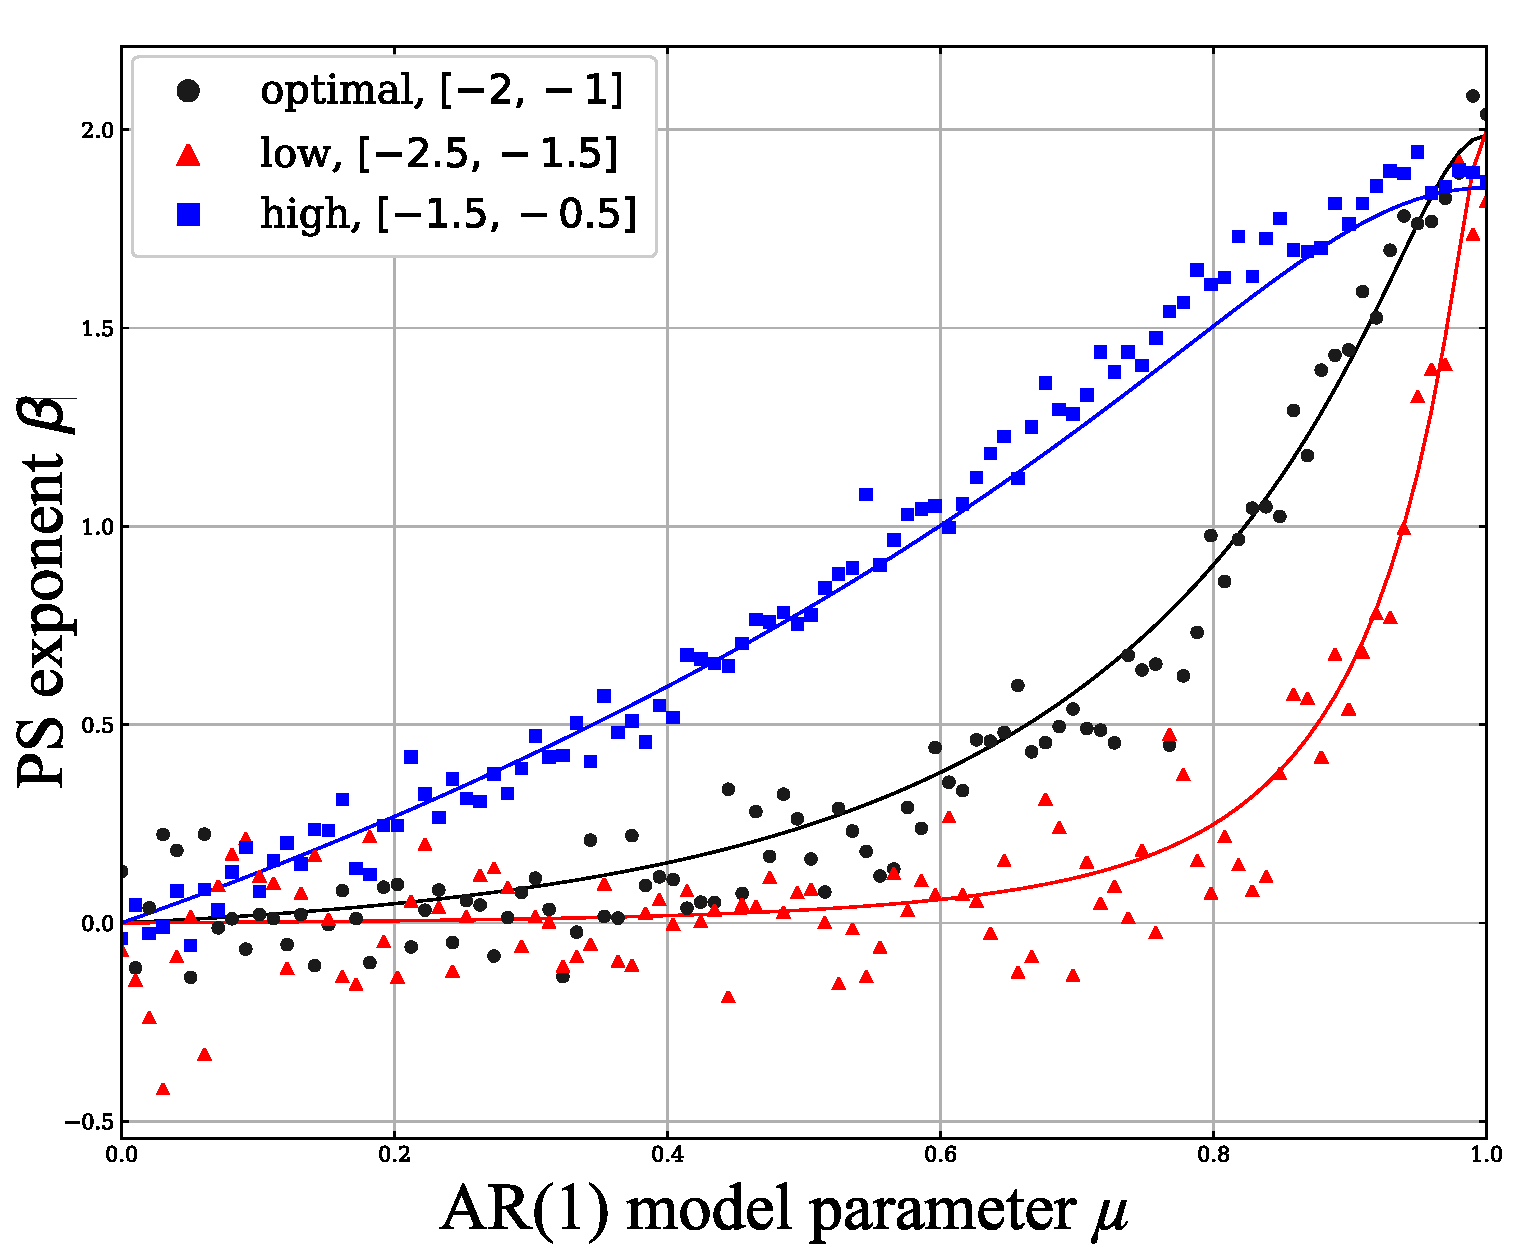
\includegraphics[width=0.95\linewidth]{c2fig07mod}
	\caption{\label{fig:1D:PSestimate}
		{The PS exponent $\beta$ estimated for 100 AR(1) time series with $0\leq\mu\leq1$. The exponent is estimated by taking the gradient of the periodogram in a range of frequencies and three different ranges are used to give three estimates for each series: one estimate using the optimal range $\m2\leq\log(f)\leq\m1$ (circles), an estimate using a lower range of frequencies $\m2.5\leq\log(f)\leq\m1.5$ (triangles) and one using a higher range of frequencies $\m1.5\leq\log(f)\leq\m0.5$ (squares). The true value of $\beta$ as a function of $\mu$ is shown as a solid line, see Eqn.~\ref{eqn:PSintegral}.}
		}
\end{figure}

The power spectrum of the AR(1) process (Eqn.~\ref{eqn:1D:PSindicator:AR1powerspectrum}) is plotted in Fig.~\ref{fig:AR1PowerSpectrum} for various values of the auto regressive parameter $\mu$. For $\mu\in(0,1)$ the power spectrum contains a crossover point (similar the simple sum of the white noise and random walk processes in Fig.~\ref{fig:1D:crossover1}) where the power spectrum changes from a flat ($\mu=0$) shape at low frequencies to a negative-gradient ($\mu=1$) shape at high frequencies. Estimating the PS scaling exponent by performing a linear fit within some range of frequencies will clearly give inconsistent results based on the range chosen, as discussed in Sec.~\ref{sec:frequencyRange}. By integrating the expression in Eqn.~\ref{eqn:PSE_calculation} over the desired frequency range $a_1\leq\log(f)\leq a_2$, we obtain an expression for the estimated value of $\beta$ (as a function of $\mu$) when using that range:
\begin{eqnarray}
		\beta &= \int_{a_1}^{a_2}-\frac{d\log\left[S_z(f)\right]}{d(\log f)}d(\log f)\nonumber\\
		&= \log\left[  \frac{1+\mu^2-2\mu \cos(2\times10^{a_2}\pi)}{1+\mu^2-2\mu \cos(2\times10^{a_1}\pi)}  \right],
		\label{eqn:PSintegral}
\end{eqnarray}
where $S_z(f)$ is the PSD of the AR(1) process given by Eqn.~\ref{eqn:1D:PSindicator:AR1powerspectrum}.

As an experiment we generate 100 AR(1) time series of length $10^5$ with different parameter $\mu$ values in the range $[0, 1]$. We then estimate the PS exponent using three frequency ranges:
\begin{itemize}
	\item The `optimal' range: ($\m2\leq\log(f)\leq\m1$).
	\item Lower frequencies: ($\m2.5\leq\log(f)\leq\m1.5$).
	\item Higher frequencies: ($\m1.5\leq\log(f)\leq\m0.5$).
\end{itemize}
The results are shown in Fig.~\ref{fig:1D:PSestimate}. We note that the PS exponent estimation accurately recreates the expected values given by Eqn.~\ref{eqn:PSintegral}. The variance (after subtracting the expected values) when using the lower frequencies is significantly larger ($0.026$) than when using the optimal range ($0.0075$) or the higher frequency range ($0.0037$), an observation attributable to the fact that the periodogram is noisier at lower frequencies, and this becomes more apparent with shorter time series. 

We also note, looking at Fig.~\ref{fig:1D:PSestimate}, that using lower frequencies yields an indicator that is more sensitive to change in AR parameter $\mu$ close to $1$ but it shows no change as $\mu$ increases from $0$ to $0.8$, as observed already with Fig.~\ref{fig:AR1PowerSpectrum}. At the end of Sec.~\ref{sec:frequencyRange} we remark that this may be useful for tipping point detection in specific systems with $\mu$ close to $1$, as confirmed here. Also with Fig.~\ref{fig:1D:PSestimate} we are able to observe the difference in behaviour for the other frequency ranges, in particular that the PS exponent increases almost linearly with $\mu$ when using higher frequencies, and this property may itself be exploited in specific cases. 


%Variances:
%Low:     0.026072720528987823
%Optimal: 0.007549882964978143
%High:    0.0036827022327993275


\section{Sensitivity analysis}
\label{sec:sensitivity}

\subsection{Sensitivity of the PS exponent to time series length}

\begin{figure}
	% plotted using the Matlab script 'PSwindowsize_sensitivity.m'
	\centering
	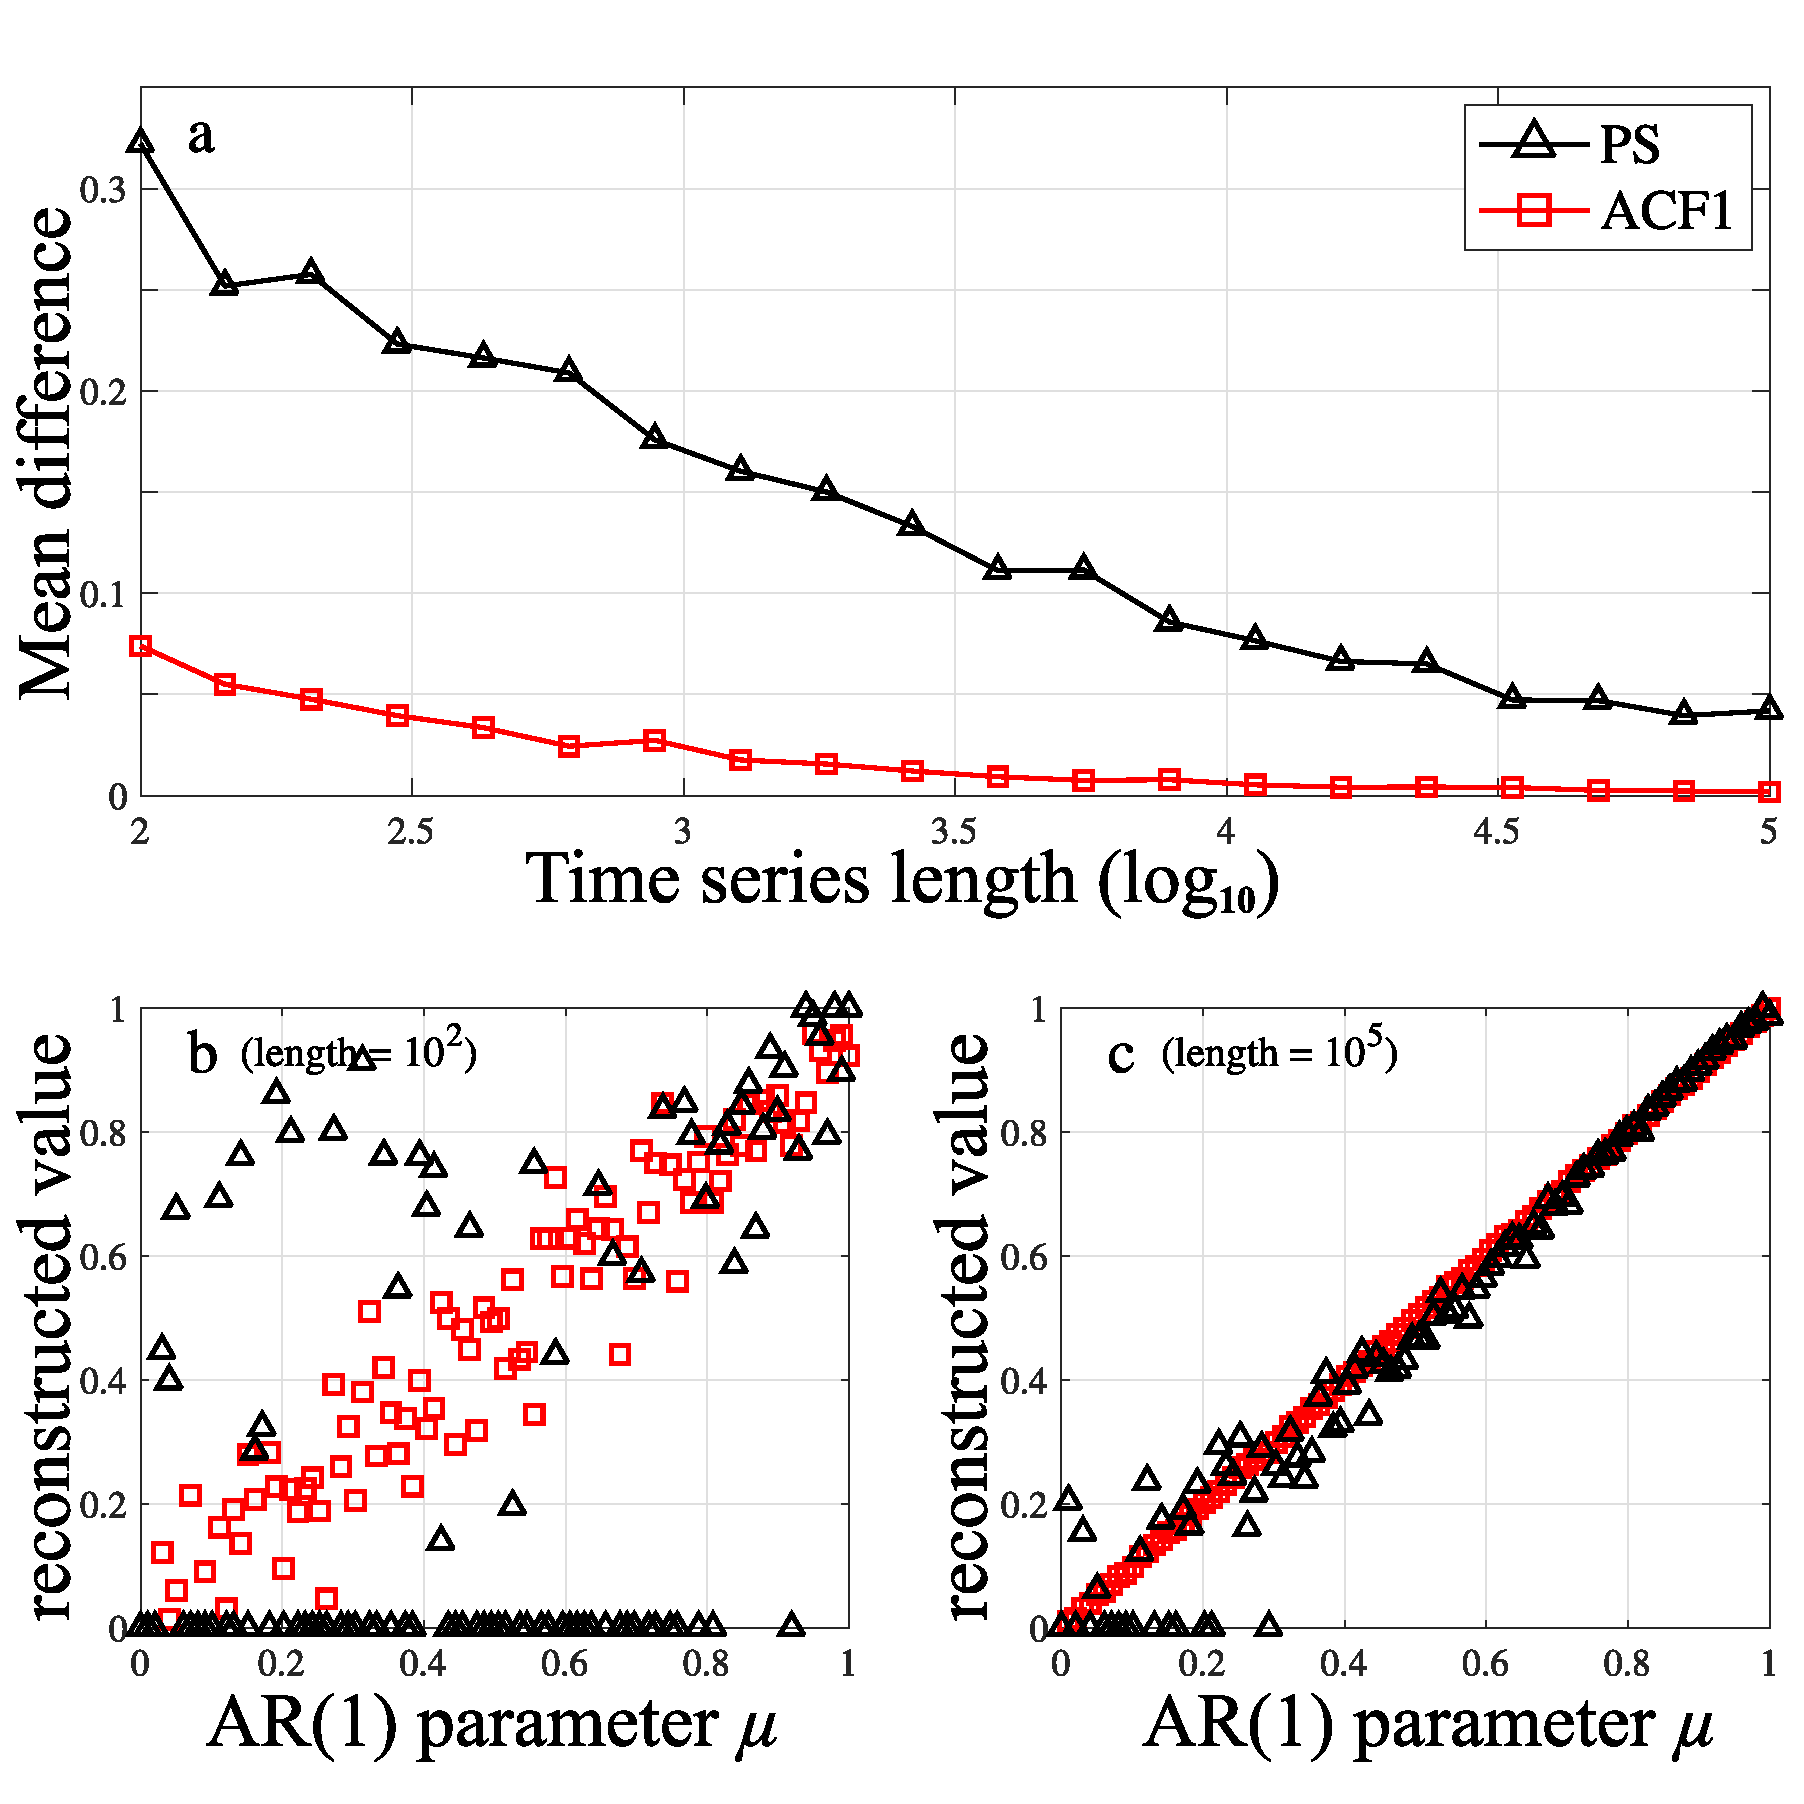
\includegraphics[width=0.9\linewidth]{c2fig12}
	\caption{\label{fig:1D:PSsensitivity}
		Sensitivity of the ACF1 and PS indicator to time series length as estimators of the AR(1) model parameter. Panel~{\bf a}: For $10^2\leq N\leq 10^5$ time series of length $N$ are created using an AR(1) model with $100$ different values of the parameter $\mu$ in the range $[0,1]$. The value of the model parameter is then estimated using either the lag-1 autocorrelation or the PS exponent $\beta$ (see equation~\ref{eqn:1D:PSindicator:reconstruct_mu_repro}). The mean difference between the estimated value and the true value is plotted for the ACF1 method (squares) and the PS method (triangles).  Panels~{\bf b},~{\bf c}: The estimated values of the parameter $\mu$ are plotted against the true values when using a series length $N=10^2$ (the shortest considered) and $10^5$ (the longest considered). Negative values of the PS indicator are mapped to $\mu=0$.
	}
\end{figure}

If we calculate the PS exponent $\beta$ using the frequency range $\m2\leq\log(f)\leq\m1$, as we have established above, then when concerned specifically with the AR(1) process we may reconstruct the value of the AR parameter $\mu$ by performing the inverse function of the $\beta$ calculation in Eqn.~\ref{eqn:PSintegral}, that is,
\begin{equation}
	\label{eqn:1D:PSindicator:reconstruct_mu_repro}
	\mu(\beta)\approx b-\sqrt{b^2-1}~, ~~ b = \frac{\cos(0.2\pi)-10^\beta \cos(0.02\pi)}{1-10^\beta}.
\end{equation}
Doing so allows us to test the accuracy of the exponent estimation by calculating the variability between the true value $\mu$ and the reconstructed value. For 100 values of $\mu$ in the range $[0,1]$ (i.e. $\mu = 0, 0.01, 0.02, ...$) we produce a time series of a given length using an AR(1) process for each of the parameters $\mu$. We then calculate the mean difference (over the 100 values) between the true value $\mu$ and the reconstructed value obtained from the PS exponent $\beta$. The results are shown in Fig.~\ref{fig:1D:PSsensitivity} where the mean difference is plotted for different time series lengths, alongside the standard method to estimate the AR parameter: the simple lag-1 autocorrelation function (ACF1). We see that the PS exponent is a poor proxy for autoregressive parameter in comparison to the ACF1 estimator, {\revision particularly} for short time series, although the gap does narrow with increasing time series length. This poses a problem for the use of the PS exponent as a tipping point indicator where the value is calculated in a short (comparatively to the scale on which the tipping takes place) sliding window. 


\subsection{Sensitivity of the PS exponent to trends}

Despite the accuracy of the ACF1 estimator in reconstructing the value of the AR(1) parameter (in comparison to the PS exponent), there are some situations in which the ACF1 is less suitable as a tipping point indicator. For example, when trends or oscillations are present in a time series these must be removed before calculating the autocorrelation since they create a high ``background correlation'' against which it is difficult to measure an increase in the vicinity of a tipping point~\cite{prettyman2019}. It may be the case, however, that removing oscillations at multiple frequencies is difficult and doing so destroys some of the increasing correlation one is hoping to detect (see Ref.~\cite{prettyman2021} pp.175-178). 

The measurement of the PS exponent, by its nature, is likely to be resilient to oscillations in the time series since oscillations at specific frequencies will show as short spikes in the periodogram which will be averaged-out when taking the negative gradient. Moreover, if logarithmic binning is used to preprocess the periodogram before the estimation (in order to remove the bias in favour of high frequencies) many such spikes will likely be removed\footnote{For particulars of this logarithmic binning, see Ref.~\cite{prettyman2021} p.48, p.89}. In this section we investigate this resilience, both to oscillations and to a non-linear trend. 

We now consider an AR(1) process with added parabolic trend, given by the equation 
\begin{equation}
	X(t_{n}) = \mu X(t_{n-1}) + \eta_n + 5t_n^2\,,
\end{equation} 
where $[t_1,\dots,t_N] = [0,\dots,1]$ and the $\eta_n$ are independent Gaussian white noise terms. The trend will tend to increase the autocorrelation in the resulting time series and, in a practical tipping-point detection context, would be removed by subtracting a polynomial fit before analysis. We then repeat the experiment shown in Fig.~\ref{fig:1D:PSsensitivity}, calculating the mean difference between the true value $\mu$ and the value reconstructed from the PS exponent $\beta$, besides the ACF1 estimator, for a range of values $\mu\in[0,1]$. The results are shown in Fig.~\ref{fig:1D:PSsensitivity_trend}. The constant high (in comparison to the case with no trend) value for the ACF1 estimator is explained by the fact that the ACF1 consistently \emph{over}-estimates the AR(1) parameter where $\mu<0.9$. The PS exponent also over-estimates the value in short time series, giving a constant value $1$, as shown in Fig.~\ref{fig:1D:PSsensitivity_trend}{\bf b}. But for series longer than $10^3$ the PS exponent actually performs better than the ACF1 estimator. Indeed, we note the similarity between Fig.~\ref{fig:1D:PSsensitivity_trend}{\bf c} and Fig.~\ref{fig:1D:PSsensitivity}{\bf c} (using time series of length $10^5$ in both cases): it appears that for time series length $N=10^5$ the trend does not affect the PS indicator at all. 

{\revision The PS indicator will, therefore, be most useful as an EWS in cases where a tipping point occurs over a period of $\geq 10^3$ points - e.g. on a scale of months where
	hourly data are available, which is the case for some meteorological datasets from recent decades \cite{HadISD, NOAAcoralreefdatabase}. This raises the possibility of detecting modern weather- and climate-related tipping points such as coral bleaching \cite{hoegh2007coral, goreau2021global} which is linked to increase in ocean temperatures. }

\begin{figure}
	% plotted using the Matlab script 'PSwindowsize_sensitivity.m'
	\centering
	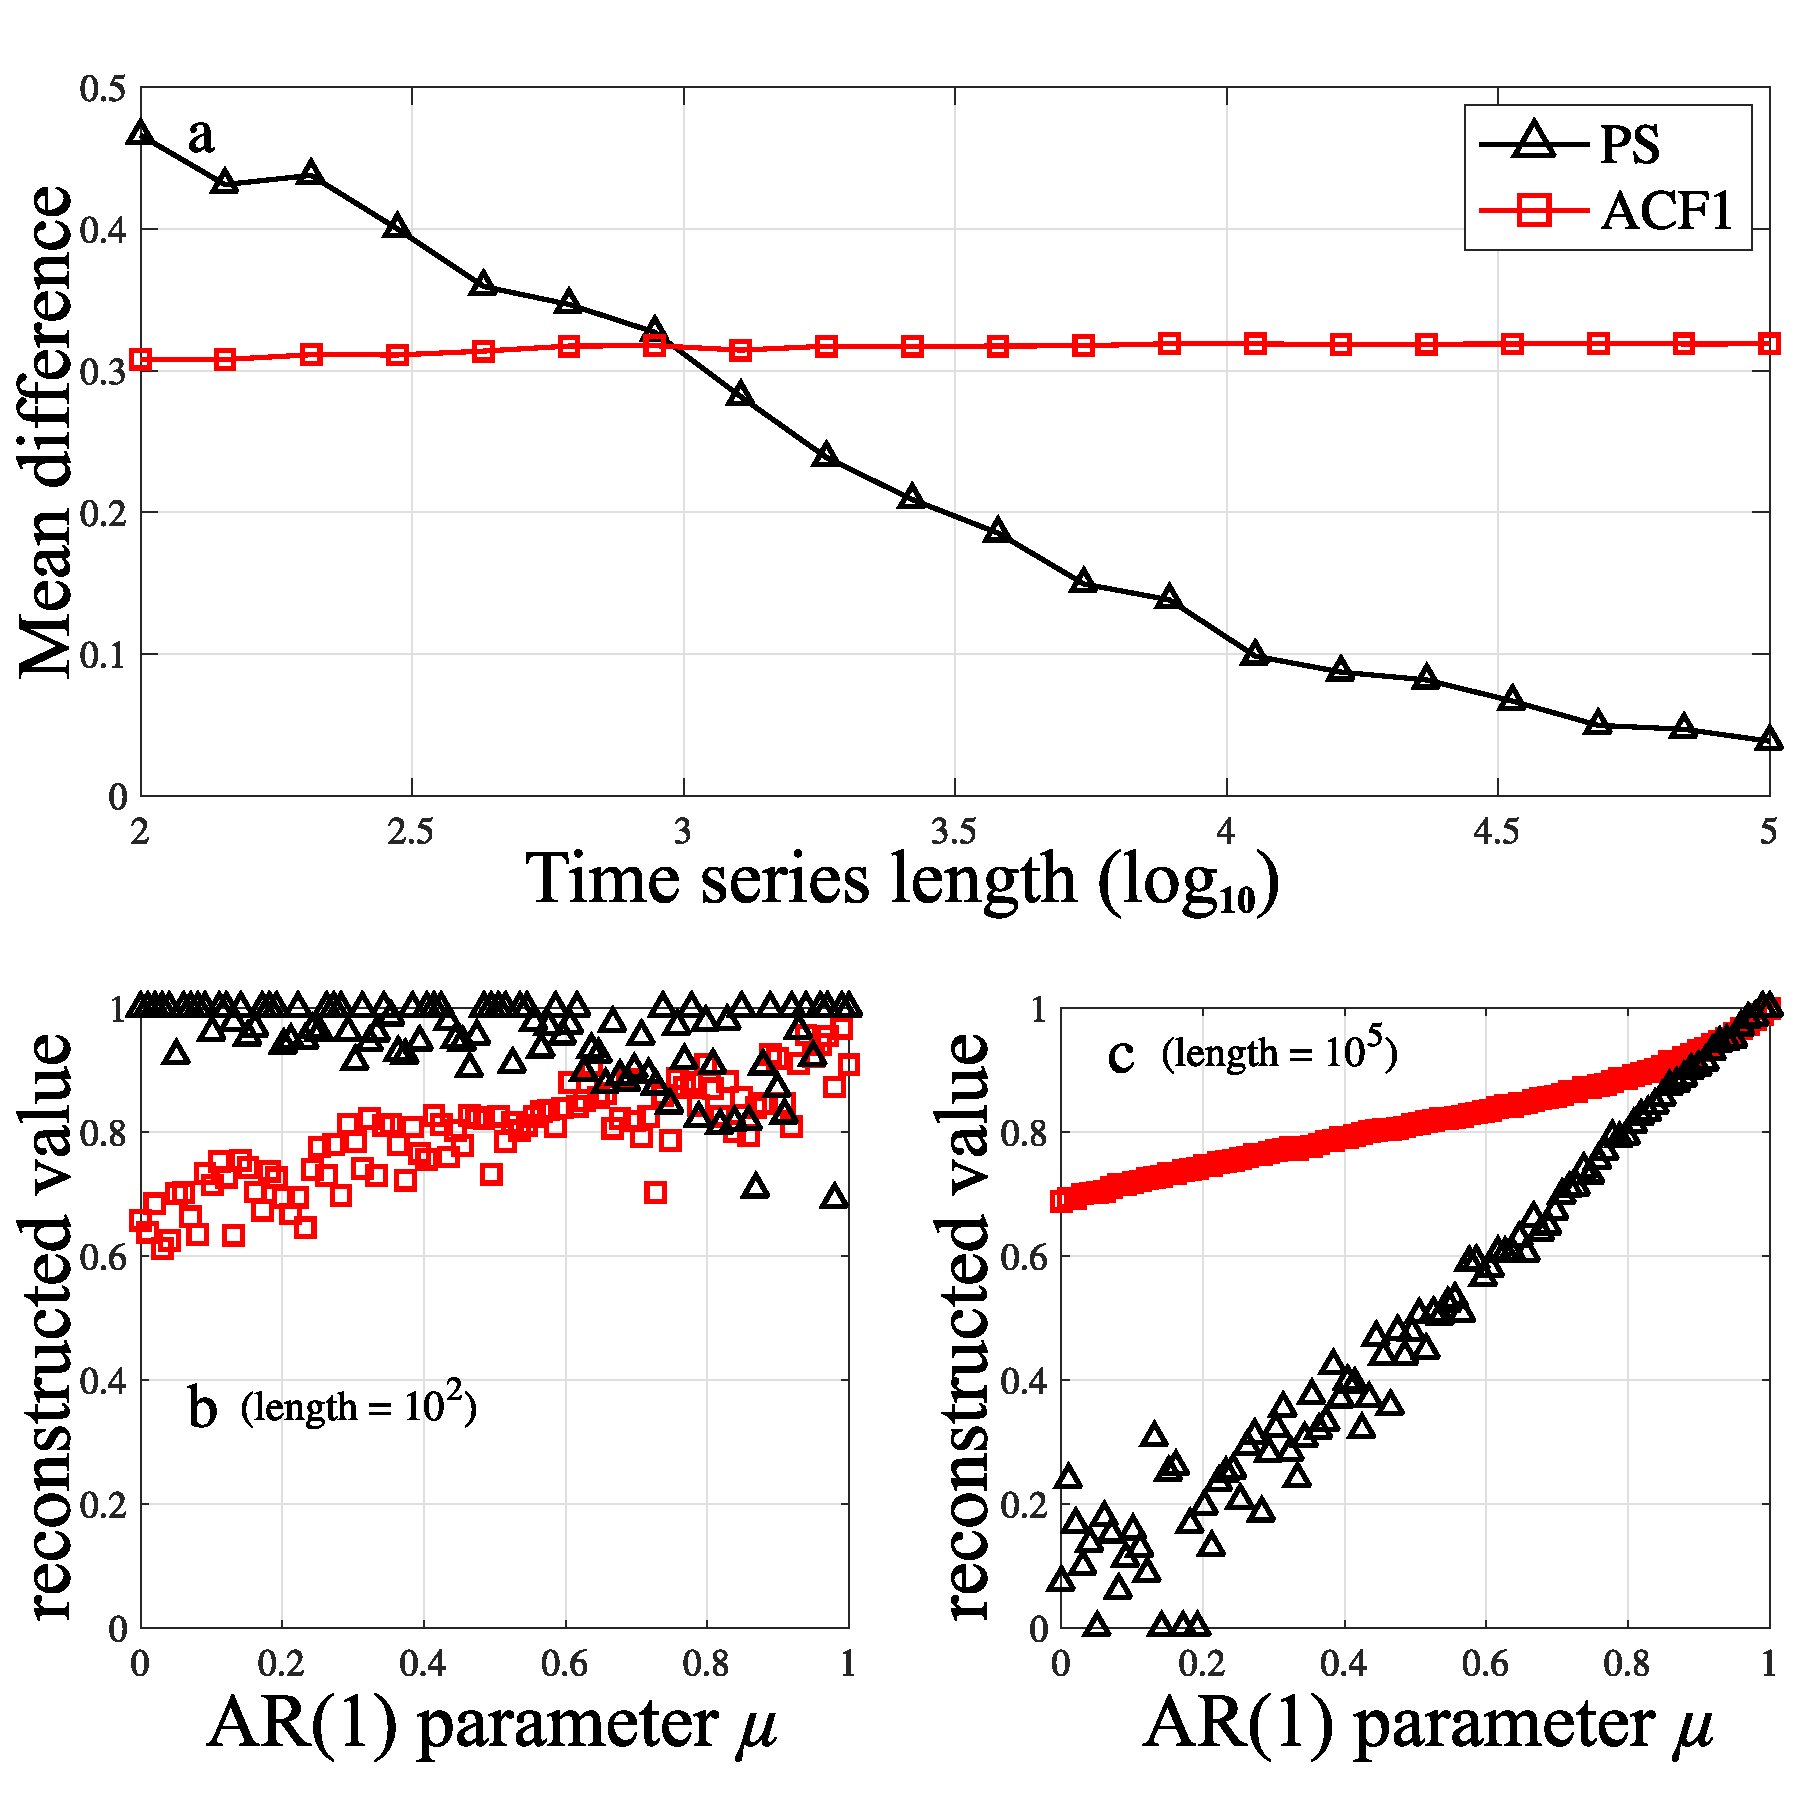
\includegraphics[width=0.9\linewidth]{c2fig14}
	\caption{\label{fig:1D:PSsensitivity_trend}
		Sensitivity of the ACF1 and PS indicator to time series length as estimators of the AR(1) model parameter when a parabolic trend is added to the AR(1) process. Panel~{\bf a}: For $10^2\leq N\leq 10^5$ time series of length $N$ are created using an AR(1) model with a parabolic trend with $100$ different values of the parameter $\mu$ in the range $[0,1]$. The value of the model parameter is then estimated using either the lag-1 autocorrelation or the PS exponent $\beta$. The mean difference between the estimated value and the true value is plotted for the ACF1 method (squares) and the PS method (triangles).  Panels~{\bf b},~{\bf c}: The estimated values of the parameter $\mu$ are plotted against the true values when using a series length $N=10^2$ (the shortest considered) and $10^5$ (the longest considered).
	}
\end{figure}



\subsection{Sensitivity of the PS exponent to periodicity}

Besides the long-term parabolic trend considered above, we also consider the addition of a periodic function to the AR(1) model. To this end we superimpose a simple sine wave, or combination of sine waves, over an AR(1) process $Z(t)$ with parameter $\mu$: that is, 
\begin{equation}
	Z(t_k) = \mu Z(t_{k-1}) + \eta_k\,,
\end{equation}
where the $\eta_k$ are i.i.d. Gaussian white noise terms. As an experiment we use time series of length $N=10^4$ with time variable $t\in[0,20\pi]$ (so that $t_0=0$, $t_N=20\pi$) to create three distinct time series:
\begin{enumerate}
	\item The original time series $z(t) = Z(t)$.
	\item The original time series plus a simple sine wave $z(t) = Z(t) + \sin(t)$.
	\item The original time series plus a more complicated function $z(t) = Z(t) + 2\sin(50t)+3\sin(7t)$.
\end{enumerate}
Since the time variable is in the range $[0,20\pi]$, ten periods of the function $\sin(t)$ occur within the time series in each case, whilst $500$ and $70$ periods of the functions $2\sin(50t)$ and $3\sin(7t)$ occur respectively. Using the same method as the experiments shown in Figs.~\ref{fig:1D:PSsensitivity}\&\ref{fig:1D:PSsensitivity_trend} we create the three groups of time series 100 times using different values of $\mu\in[0,1]$, and for each of the $3\times100$ time series we calculate the lag-1 autocorrelation function (ACF1), the DFA exponent (see Refs.~\cite{kantelhardt2001, livina2007}) and the PS exponent. The results are shown in Fig.~\ref{fig:1D:periodicity:sineWaveAR1} which also shows the expected values for the ACF1 (straight line) and PS exponent (curve given by Eqn.~\ref{eqn:PSintegral}). 

We note that when the periodic functions are added to the AR1 series the same over-estimation occurs in the ACF1 estimator as observed in Fig.~\ref{fig:1D:PSsensitivity_trend}{\bf b},{\bf c}. The DFA exponent also suffers the same deficiency as we observe the difference between the DFA exponents plotted in column {\bf a} (pure AR(1) process) and those in columns {\bf b} and {\bf c}. If, however, we observe the bottom row of Fig.~\ref{fig:1D:periodicity:sineWaveAR1} in which the PS exponents are plotted. There is no noticeable difference between the three columns. The PS indicator is robust under the influence of periodicities in the time series. 


\begin{figure}
	% plotted using the Matlab script 'sineWaveAR1.m'
	\centering
	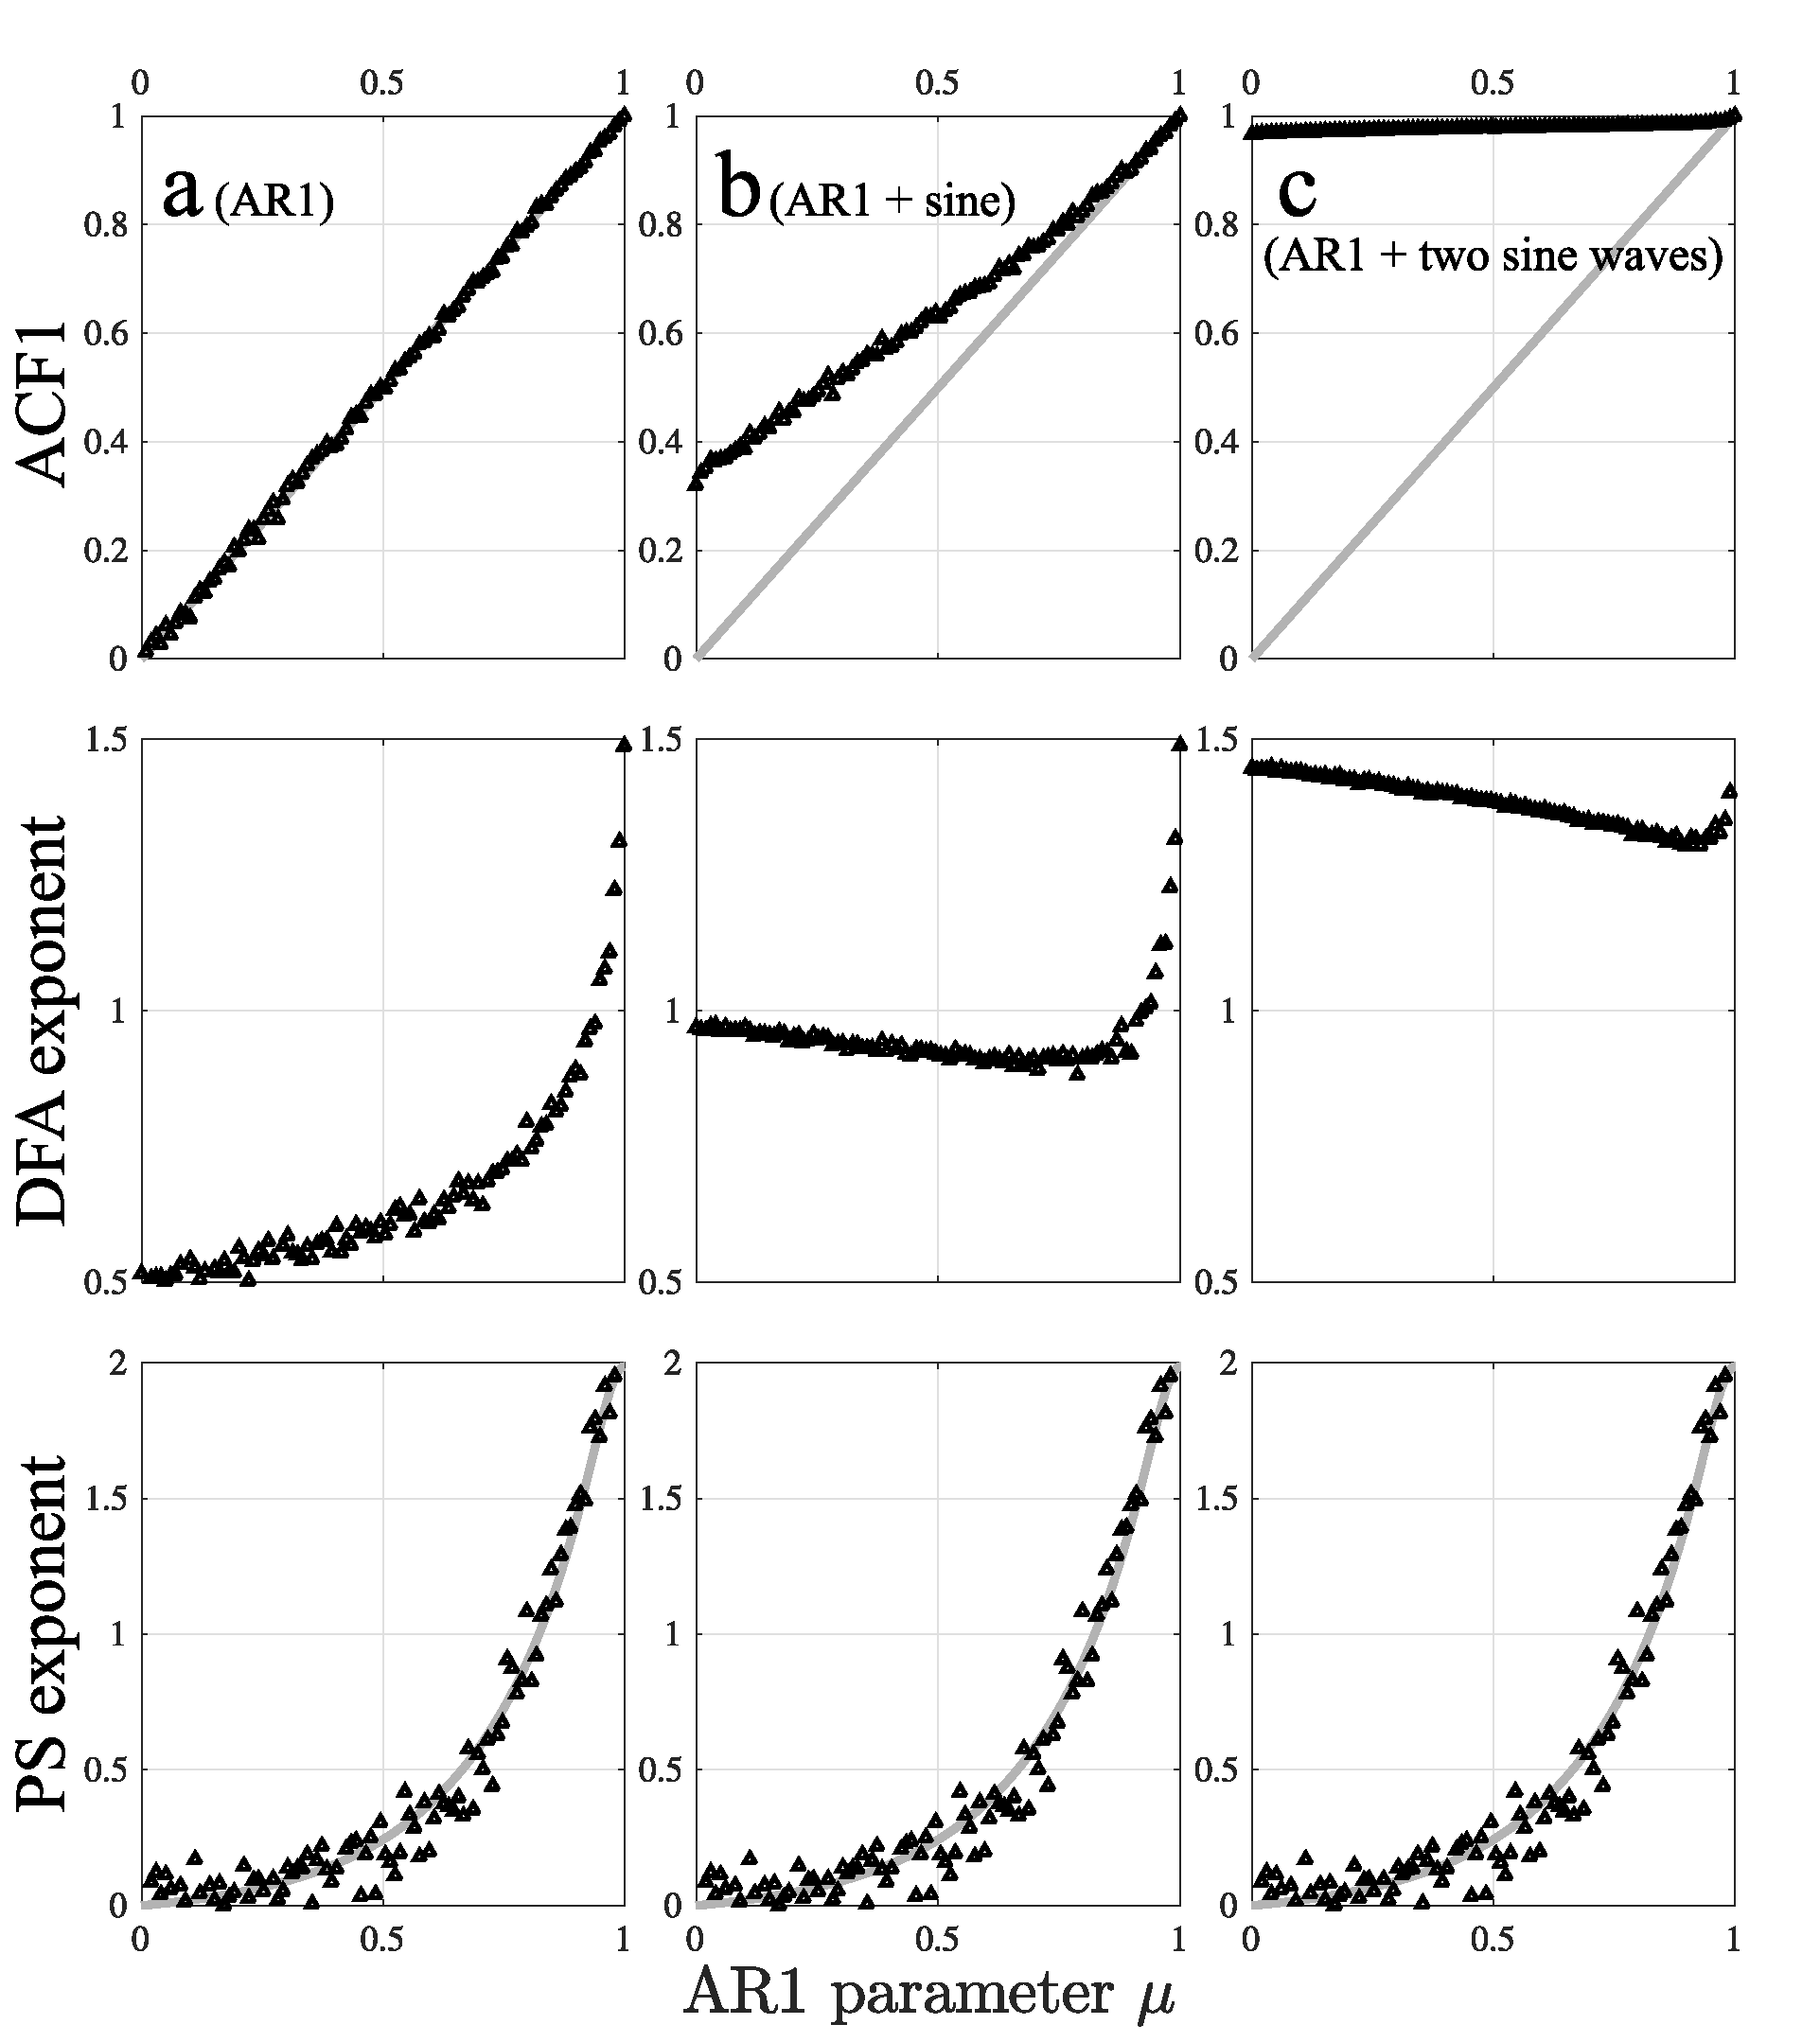
\includegraphics[width=0.9\linewidth]{c2fig19_sineWaveAR1}
	\caption{\label{fig:1D:periodicity:sineWaveAR1}
		The ACF1 (top row), DFA exponent (middle row) and PS exponent (bottom row) are calculated for $100$ AR(1) time series of length $10^4$ with $\mu\in[0,1]$. The AR(1) time series is superimposed with either no other function (column {\bf a}), a simple sine wave (column {\bf b}), or a more complicated periodic function (column {\bf c}). We note that the PS exponent is practically the same in all three cases and is not affected by periodicities. In the case of the ACF1 and PS, the expected value function is plotted in grey.
	}
\end{figure}



\section{An application to GISP ice-core data}
\label{sec:gisp-ice-core}

{\revision
Although the results in Fig.~\ref{fig:1D:periodicity:sineWaveAR1}, where the PS exponent value closely matches the analytically-derived value, require a window of $\geq 10^3$ data points, it is possible to detect an increase in the PS indicator prior to a tipping point with much shorter time-series \cite{prettyman2019}. We here attempt to approximate the results obtained by Ref.~\cite{lenton2012climate}\footnote{see Fig.~3 in this reference} where the DFA and ACF-1 indicators are applied to a paleo-temperature proxy – the GISP2 $\delta^{18}O$ water isotope record from Greenland ice-cores \cite{rasmussen2008synchronization}. The PS indicator is applied to the data with a sliding window of 4kyr (approximately 200 points), which allows for the use of logarithmic binning in the PS exponent estimation but masks the slowing down which happens on a relatively short (i.e. $<100$ data points) scale. In Ref.~\cite{lenton2012climate} the B\o{}lling warming event at 14.7kyr before present is preceded by a steady rise in the DFA indicator. We note that no such EWS is visible in Fig.~\ref{fig:gisp}, indeed the PS indicator increases relatively sharply, and does so with a lag of 1kyr (50 data points) rather than preceding the tipping. The increase does, however, whilst not providing an EWS, demonstrate presence of slowing-down in the data, confirming the results of Ref.~\cite{lenton2012climate}, which are subject to debate \cite{lenton2008, ditlevsen2010}.
}

\begin{figure}
	% plotted using the Matlab script 'sineWaveAR1.m'
	\centering
	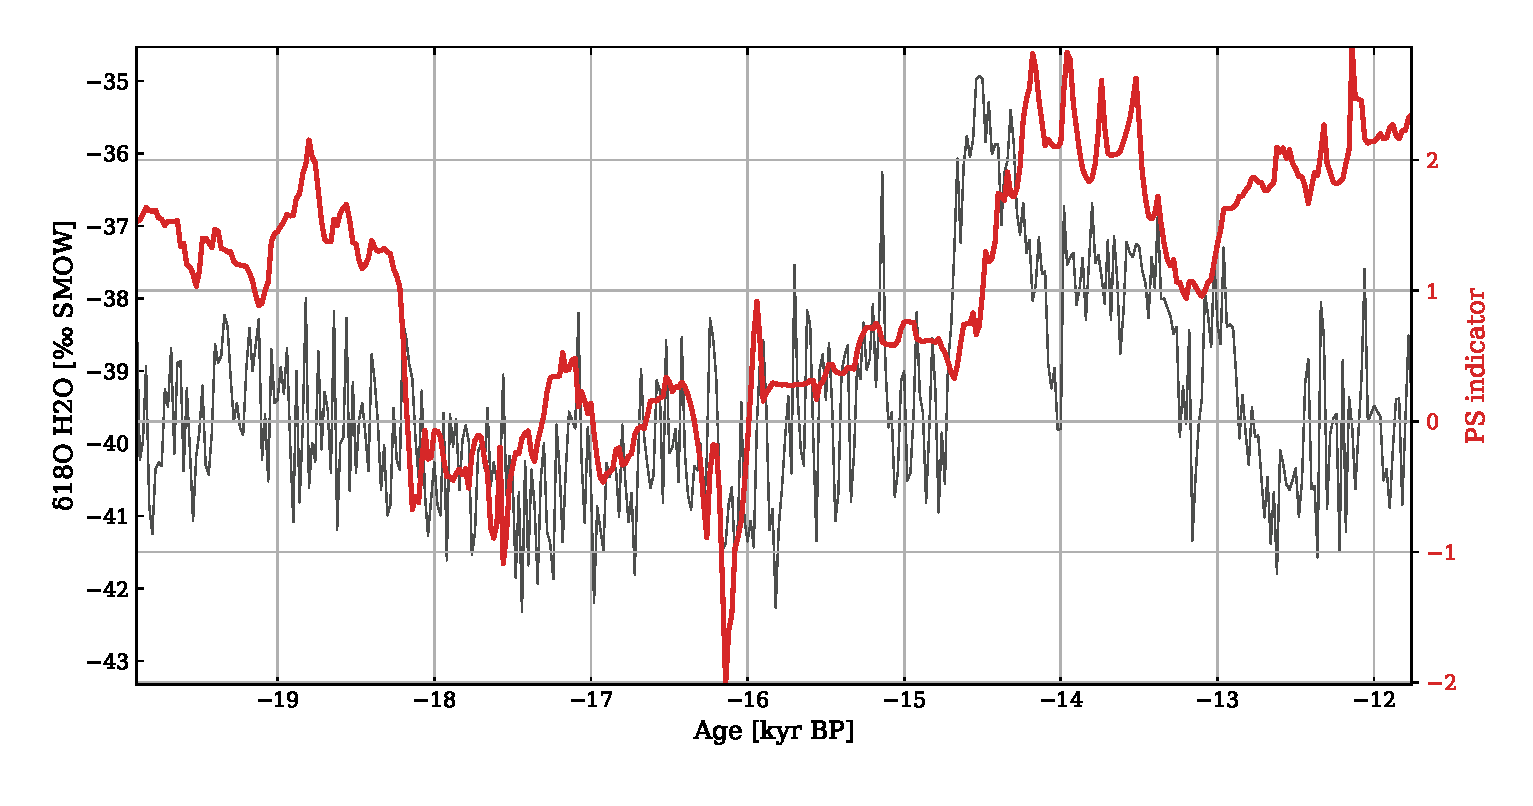
\includegraphics[width=0.9\linewidth]{GISP_fig09}
	\caption{\label{fig:gisp}
		{\revision
		The PS indicator applied to the $\delta^{18}O$ water isotope record with a sliding window of 4kyr. The B\o{}lling warming event at 14.7kyr is visible in this temperature proxy but the PS indicator is unable to provide an EWS with such low time-resolution. 
		}
	}
\end{figure}

\section{Summary}
\label{sec:Summary}

In this paper we have studied the use of the power spectrum scaling exponent as a tipping point indicator (Sec.~\ref{sec:modellingCSD}) and obtained several key results regarding the implementation of such a technique. 

In particular, in Sec.~\ref{sec:frequencyRange} we have determined the optimal frequency range in which to estimate the PS exponent from the discrete periodogram, based on using the AR(1) process as a model of critical slowing down. We note, however, that there may be certain systems for which it is informative to use a different frequency range. 

In Sec.~\ref{sec:noTrueScaling} we have then shown that it is worthwhile (chiefly considering the AR(1) process) to estimate the PS exponent even when the power spectrum does not exhibit true power-law scaling since, when applying the PS indicator to dynamical systems with tipping behaviour, it is not the exact value of the indicator that is of interest but the change in the value over time as the indicator is applied in a sliding window on the time series. In particular we are concerned with the detection of critical slowing down in the time before a tipping point is reached, which is characterised by an increase in the autocorrelation (for which the PS exponent is a proxy) or, in other words, a ``reddening'' of the power spectrum as the return time around a stable state increases. 

In Sec.~\ref{sec:sensitivity} we then demonstrate two key differences in behaviour between the PS exponent and the simple lag-1 ACF in detecting a change in the AR(1) model parameter. First, that in short time series the PS exponent performs poorly (by comparison) as an estimator for the return time which, however, should not affect the usefulness of the PS exponent as a tipping point indicator. And even for longer times series ($N=10^5$) the lag-1 ACF is more accurate. We then proceed to show that when the AR(1) process is superimposed with a trend (we have used a parabolic trend) or an oscillation (the sum of sine waves), the PS exponent value is unchanged from the values obtained without the addition of a trend or oscillation. This is significant improvement over the ACF1 estimator, or even the DFA exponent which is inherently robust against low-order polynomial trends~\cite{kantelhardt2001} but cannot remove short-wavelength oscillations. This property makes the PS exponent a valuable addition to the canon of tipping point indicators in specific cases where the times series are sufficiently long and where removing oscillations or trends may be difficult or may affect the detection of EWS in real systems. This is of particular value in various ecological and geophysical systems with seasonal or diurnal periodicities, whose resilience the PS indicator may estimate with better accuracy than other techniques. 

{\revision
In Sec.~\ref{sec:gisp-ice-core} the PS indicator is able to suggest the presence of CSD in the GISP2 $\delta^{18}O$ water isotope record prior to the B\o{}lling warming event, confirming the result of Ref.~\cite{lenton2012climate}, but is not able to provide an EWS, and we conclude the the DFA and ACF-1 indicators are more appropriate in such applications. Future research involving modern high-resolution meteorological data may provide an application for the PS indicator in climate-linked tipping events over recent decades, such as coral bleaching. }

%\section*{Supplementary Material}
%\label{sec:Supplementary}
%


\section*{Acknowledgements}
\label{sec:Acknowledgements}

This paper is the result of a PhD project supported by the EPSRC Mathematics of Planet Earth centre for doctoral training, the National Physical Laboratory and the NERC National Centre for Earth Observation.


\vspace{0.5cm}
\bibliographystyle{acm}
\bibliography{bibliography_prettyman.bib}

\end{document}

